\documentclass[11pt]{article}

\usepackage{mystyle}


\spacing{1.5}
% \setlength{\parindent}{0pt}

% 스타일 기반 Text to 3D Furniture Object
\title{User Guided Style-based 3D Furniture Object Generation}
\author{anonymous}
\date{}

\begin{document}
\maketitle
\tableofcontents

\section{Motivation}
최근 1인 가구가 증가함에 따라 인테리어에 대한 관심도 높아지고 있다. 하지만 인테리어를 처음 접하는 사람들은 어떤 인테리어 스타일의 가구를 선택해야 할지, 어떤 색상의 가구를 배치해야할지 결정하기 어렵다. 또한, 가구를 실제로 구매하기 전에는 가구가 어떻게 배치될지 상상하기 어렵다. 이러한 문제를 해결하기 위해, 본 프로젝트에서는 사용자가 입력한 텍스트를 기반으로 3D 가구 객체를 생성하는 방법을 제안한다. 이 방법은 사용자의 입력으로 통해 원하는 스타일의 가구를 3D 객체로 생성해줄뿐만 아니라, 각 스타일 별로 주로 사용되는 색을 분석하여 자동으로 가구들의 색상을 매치시켜준다. 또한, 생성된 3D 가구 객체와 함께 가구의 적절한 크기도 함께 생성되며, 해당 객체를 3D 그래픽 툴을 통해 사용자가 원하는 공간에 배치할 수 있도록 obj, mtl 등의 확장자로 저장할 수 있다.

\section{Related Work}
\subsection{Text to 3D Object Generation}
% shap-e 언급

\section{Dataset}
\subsection{Color Analysis Dataset}
각 인테리어 스타일 별로 주로 사용되는 색상을 분석하기 위해 다양한 인테리어 스타일의 이미지들을 수집하였다. 오늘의 집\cite{todayhouse}의 스타일 카테고리를 참고하여 다음과 같은 7가지의 대표적인 인테리어 스타일을 선정하였다: Antique, Modern, Natural, Northern European, Romantic, Traditional Korean Style, Vintage. unsplash\cite{unsplash}, pexels\cite{pexels}, pixabay\cite{pixabay}에서 각 스타일 별로 100장 이상의 이미지를 크롤링하였다.

\subsection{Size Prediction Dataset}
가구의 적절한 크기를 예측하기 위해 3D-Front\cite{fu20203dfront} 데이터셋을 사용하였다. 3D-FRONT는 다양한 가구가 배치되어 있는 3D 공간을 제공하는 데이터셋으로, 각 가구의 크기 정보가 포함되어 있다. 또한 각 가구의 클래스 정보도 포함되어 있어, 가구의 종류에 따라 적절한 크기를 예측하는데 사용할 수 있다. 본 프로젝트에서는 3D-FRONT 데이터셋에서 제공하는 가구의 이미지와 크기 정보를 활용하여 가구의 크기를 예측하는 모델을 학습하였다.

\section{Method}
\subsection{Dominant Color Extraction by Styles}
사용자의 입력으로부터 인테리어에 사용할 색상을 결정하기 위해 인테리어 스타일 별로 주로 사용되는 색상을 분석하였다. 
k-means 클러스터링, Mean-Shift 클러스터링, DBSCAN의 방법으로 대표 색상 5개를 추출해보고 각 추출 방법의 결과를 정성적으로 비교하였다.
또한, RGB, HSV 색 공간에서의 Color Histogram을 비교하여 어떤 인테리어 스타일간의 거리를 분석하였다.

\begin{equation}
    \label{eq:color_extraction}
    \mathcal{S}^{style} = \left[ \mathbf{c}^{style}_1, \mathbf{c}^{style}_2, \cdots , \mathbf{c}^{style}_k \right]= \text{ExtractDominantColors}(\mathbf{I}^{style}, k) ,
\end{equation}
여기서 $\mathcal{S}^{style}$은 스타일 별로 추출된 대표 색상들, $c^{style}_i$는 $i$번째 Dominant Color, $\mathbf{I}^{style}$은 스타일 별로 수집된 이미지, k는 추출할 대표 색상의 개수이다.

\subsection{Text Finetuing for Furniture Generation}
사용자가 입력을 기반으로 가구들에 대한 설명을 생성하기 위해 ollama에서 Llama3.2-vision:11b\cite{touvron2024llama3}를 사용하였다. 프롬프트 엔지니어링을 통해서 사용자가 입력한 텍스트를 기반으로 가구에 대한 설명을 생성하도록 모델을 파인튜닝하였다. 
예를 들어, "A modern room contains round items"와 같은 입력이 주어지면, 모델은 해당 스타일과 색상을 반영한 가구를 생성하기 위한 텍스트를 아래와 같이 생성한다:
\begin{quote}
    "Create a modern glass table with round shape", \\
    "Create a modern wooden chair with round backrest", \\
    \dots,
\end{quote}
이렇게 생성된 텍스트는 3D 객체 생성을 위한 입력으로 사용된다. 또한, 생성된 가구의 종류는 3D-FRONT 데이터셋에서 제공하는 가구의 클래스 정보와 매칭되어, 가구의 크기를 예측하는데 사용된다.

\subsection{Color aware 3D Object Generation}
3D 객체 생성을 위해 Shap-E\cite{jun2023shapegeneratingconditional3d} 모델을 사용하였다.
Shap-E 모델은 Clip\cite{pmlr-v139-radford21a}을 이용하여 텍스트를 임베딩하고 이를 기반으로 3D 객체를 생성하기 때문에, 자연어로 표현된 색은 입력으로 사용될 수 있다.
하지만 사전에 추출된 스타일별 대표 색상은 컬러 코드로 표현되기 때문에 이를 자연어로 변환하는 과정이 필요하다. 예를 들어, RGB 색상 (255, 0, 0)은 "red"로 변환될 수 있다.
정확하게 일치하지 않는 대표 색상이 있을 수 있기 때문에, RGB 공간에서 가장 가까운 색상으로 변환하는 방법을 사용하였다.
본 프로젝트에서는 대표 색상을 자연어로 변환하기 위해 148개의 색상 이름과 RGB 색상 값을 매핑한 자료를 활용하였다.
해당 자료는 matplotlib에서 제공하는 CSS/XKCD 색상 이름을 기반으로 제작하였다.

대표 색상을 자연어로 변환하는 과정은 다음과 같이 표현할 수 있다:
\begin{equation}
    \label{eq:color_to_text}
    \begin{aligned}
        \mathbf{\hat{c}}^{style}_i &= \text{argmin}_{\mathbf{c} \in \mathcal{C}} ||\mathbf{c} - \mathbf{c}^{style}_i||_2 , \\
        \mathcal{C} &= \{ \text{red}, \text{green}, \text{blue}, \ldots \} , 
    \end{aligned}
\end{equation}
여기서 $\mathbf{\hat{c}}^{style}_i$는 $i$번째 Dominant Color의 자연어 표현, $\mathcal{C}$는 색상 이름의 집합이다. 이 과정을 통해 스타일 별로 추출된 대표 색상을 자연어로 변환할 수 있다.

변환된 대표 색상 텍스트는 Shap-E 모델의 입력으로 사용되며, 사용자가 입력한 텍스트와 함께 3D 객체를 생성하는데 활용된다. 예를 들어, "A modern glass table with round shape, dominant colors are white, black"과 같은 입력이 주어지면, Shap-E 모델은 해당 스타일과 색상을 반영한 3D 의자 객체를 생성한다.

\subsection{Furniture Size Prediction}
가구의 적절한 크기를 예측하기 위해서는 가구를 설명하는 텍스트와 가구의 크기를 매칭하는 데이터셋이 필요하다. 
하지만 그러한 데이터셋은 존재하지 않았기 때문에, Shap-E 모델이 입력으로 이미지와 텍스트를 받는다는 점을 활용하여, 3D-FRONT 데이터셋에서 제공하는 가구의 이미지와 크기 정보를 이용하여 가구의 크기를 예측하는 모델을 학습하였다.

크기 예측 모델은 Shap-E로부터 추출된 latent feature와 가구의 종류를 one-hot 인코딩한 벡터를 concatenate하여 입력으로 사용한다.
이후에 2개의 fully connected layer를 거쳐 가구의 크기를 예측한다.

\section{Experiments}
\subsection{Dominant Color Extraction Method Comparison}
k-means 클러스터링, Mean-Shift 클러스터링, DBSCAN의 방법으로 대표 색상 5개를 추출한 결과는 다음과 같다
\begin{figure}[htbp]
    \centering
    \begin{subfigure}[b]{0.3\textwidth}
        \centering
        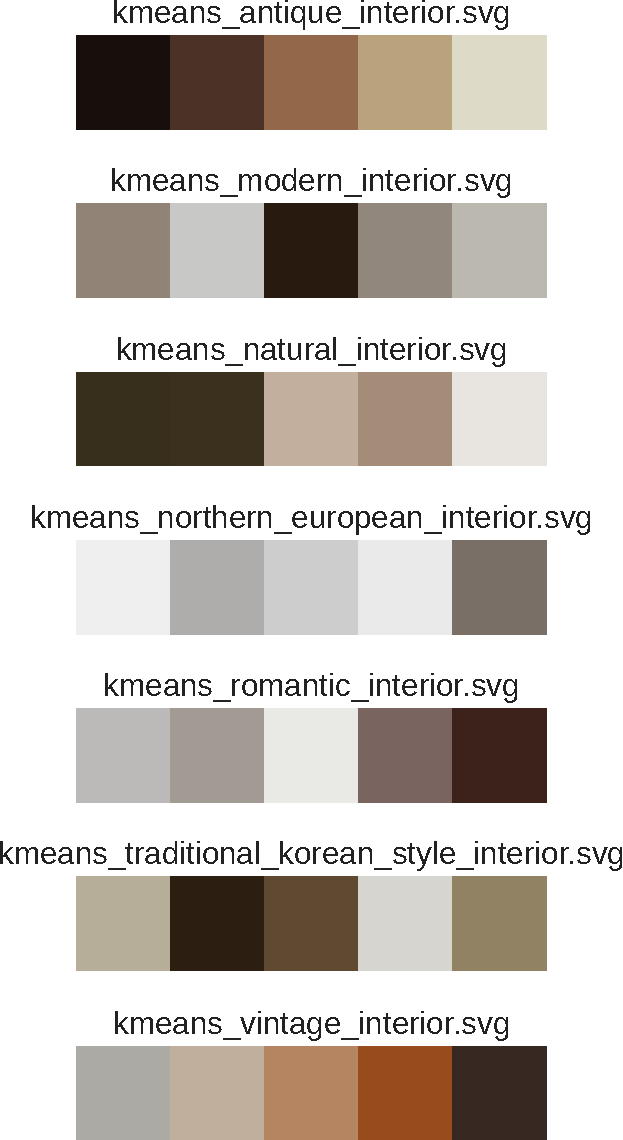
\includegraphics[height=9cm]{figures/kmeans_dominant_color.pdf}
        \caption{K-means Clustering}
        \label{fig:kmeans}
    \end{subfigure}
    \begin{subfigure}[b]{0.3\textwidth}
        \centering
        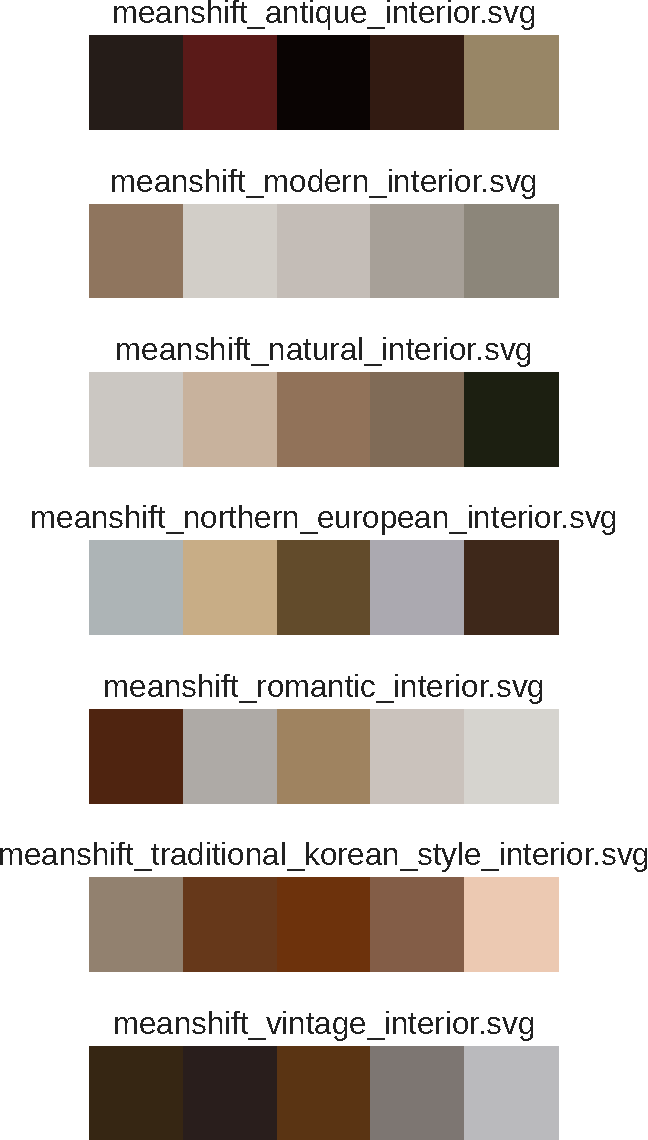
\includegraphics[height=9cm]{figures/meanshift_dominant_color.pdf}
        \caption{Mean-Shift Clustering}
        \label{fig:meanshift}
    \end{subfigure}
    \begin{subfigure}[b]{0.3\textwidth}
        \centering
        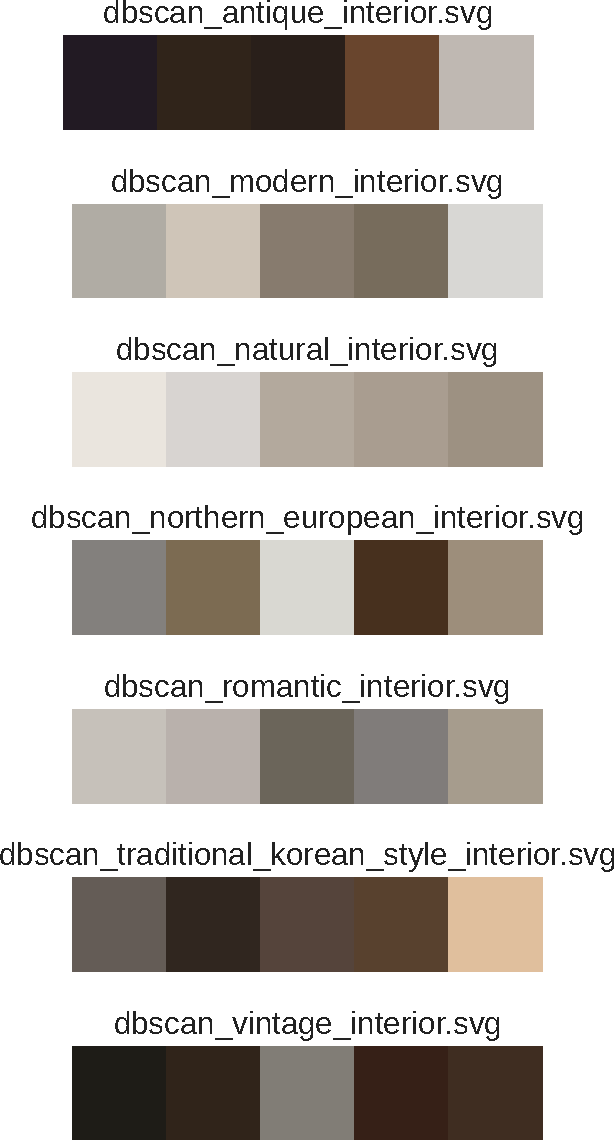
\includegraphics[height=9cm]{figures/dbscan_dominant_color.pdf}
        \caption{DBSCAN Clustering}
        \label{fig:dbscan}
    \end{subfigure}
    \caption{Dominant Color Extraction Results}
    \label{fig:dominant_color_extraction}
\end{figure}

각 색 추출 방법에 대해 정성적인 비교를 진행하였다. K-means 클러스터링은 여러 색을 다양하게 추출하면서도 인테리어의 느낌을 잘 살리는 색상을 추출하였고, Mean-Shift 클러스터링은 전체적으로 더 강한 명도의 색을 추출하였다.
DBSCAN의 경우에는 색의 다양성을 잘 살리지 못하고, 3~4개의 색상이 비슷하게 추출되는 경향을 보였다.

위와 같은 결과를 토대로 본 프로젝트에서는 K-means 클러스터링을 사용하여 대표 색상을 추출하기로 결정하였다.
\subsection{Color Histogram Comparison by Styles}
색 공간을 달리하며 색 히스토그램을 추출하고 카이제곱 거리와 바타차리야 거리를 통해 비교하였다.
\subsubsection{Color Histogram in RGB Space}
\begin{figure}[htbp]
    \centering
    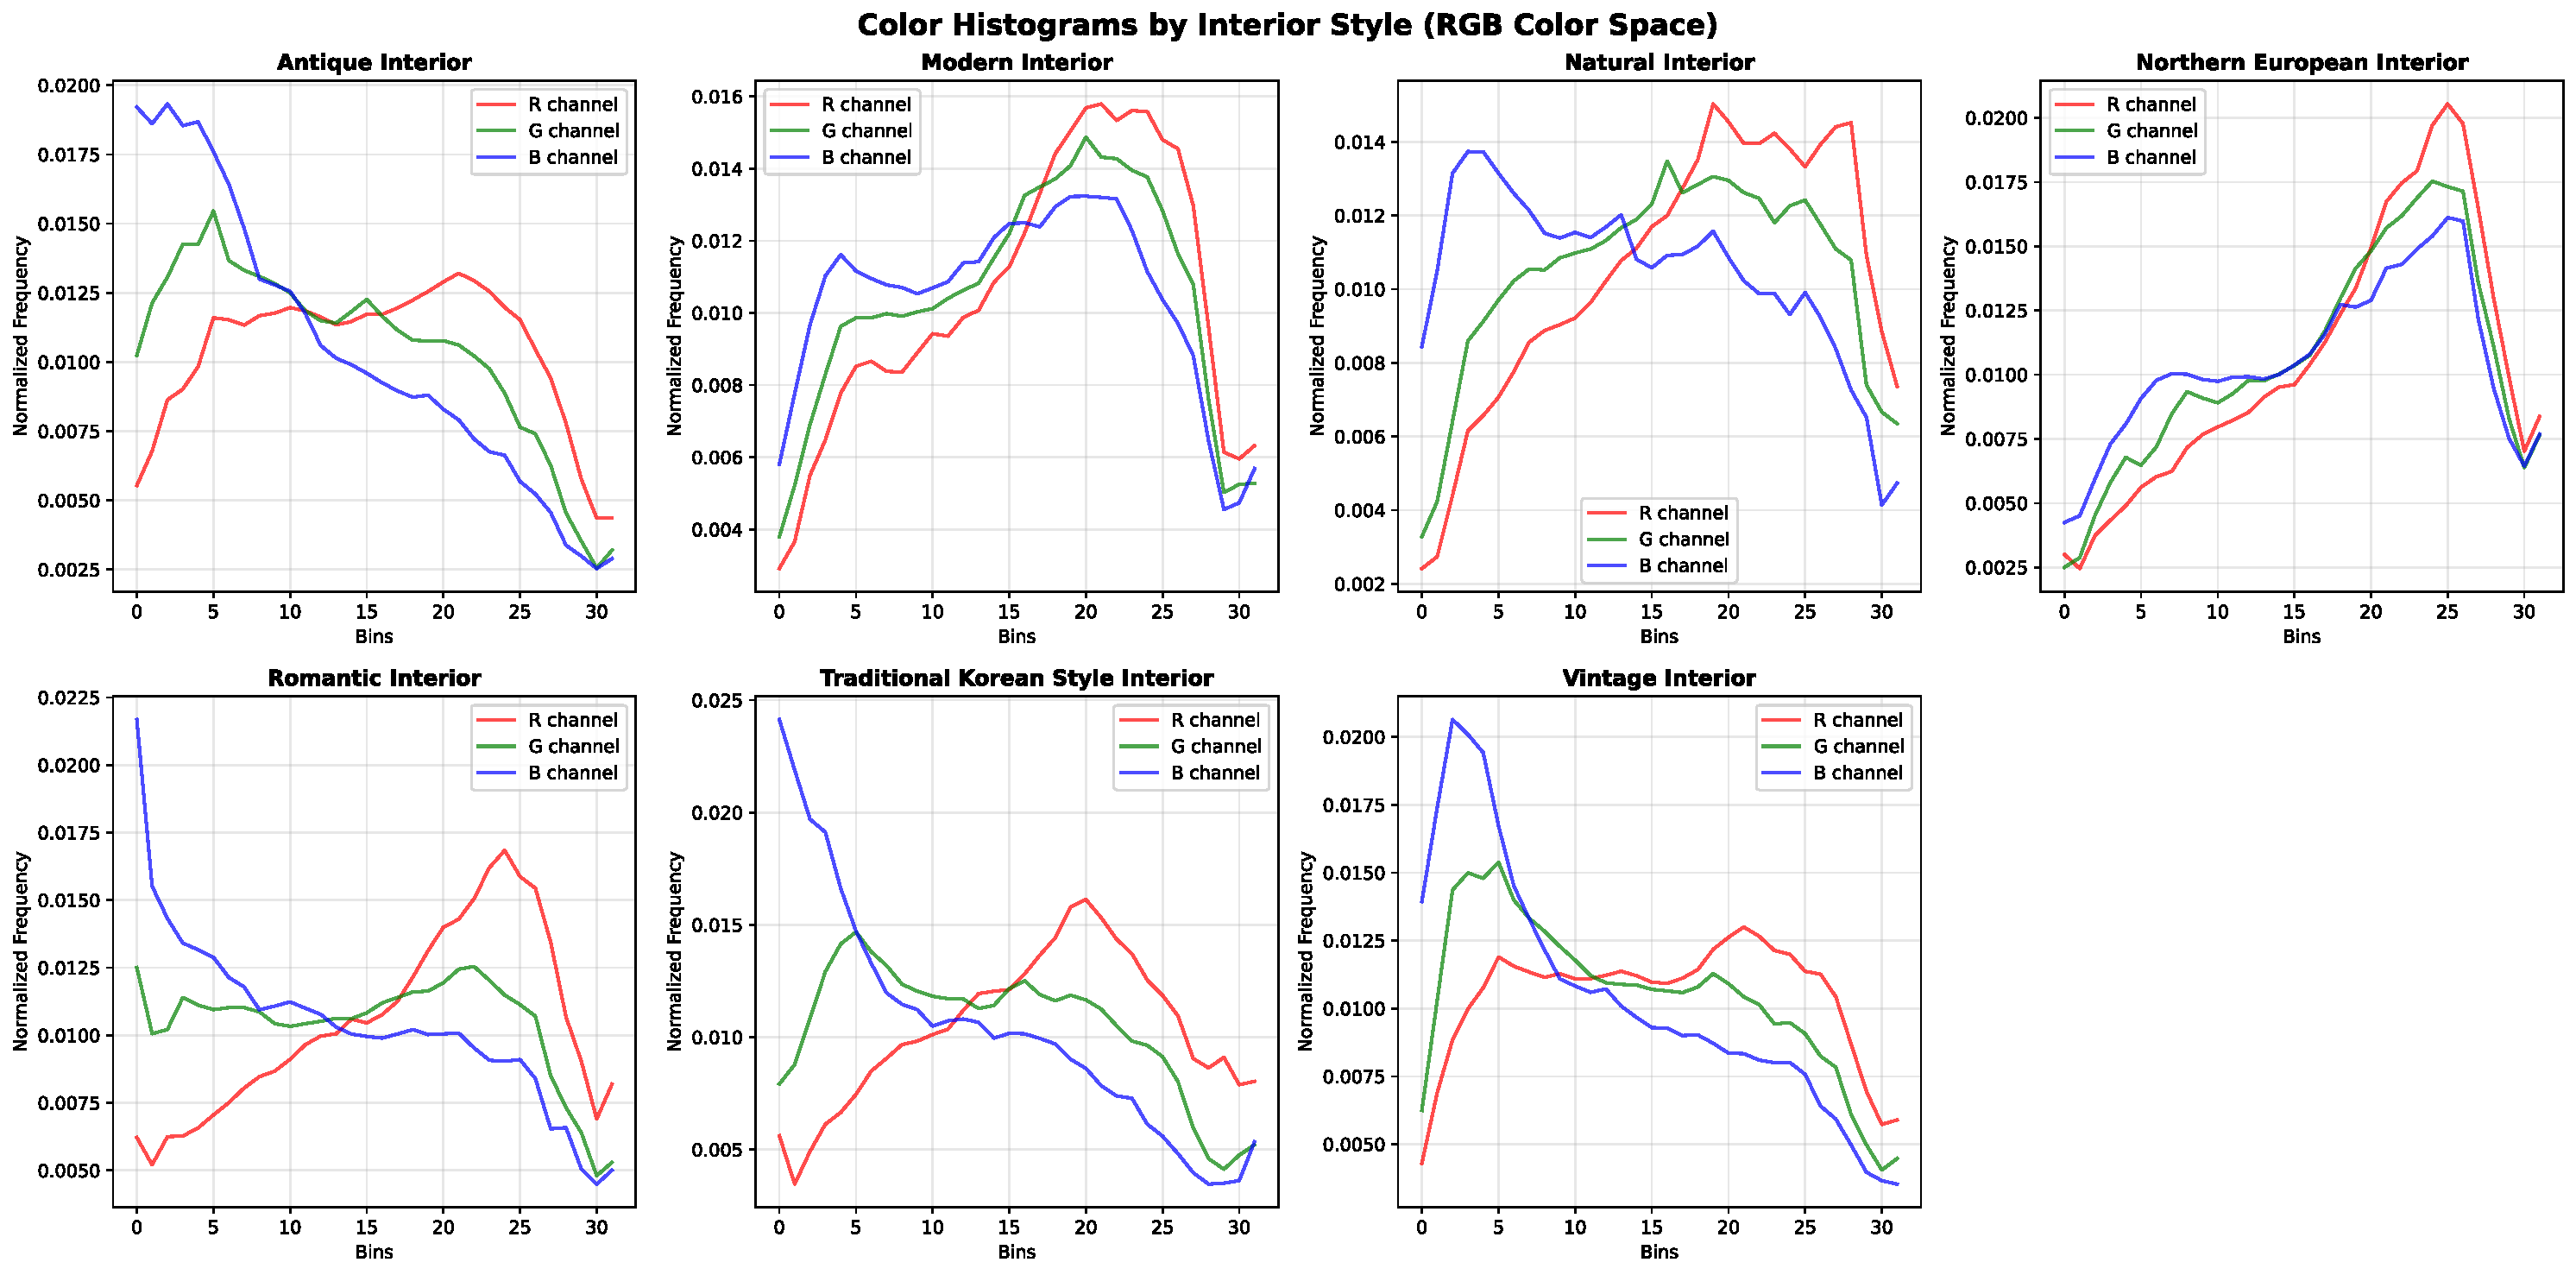
\includegraphics[width=0.8\textwidth]{figures/rgb_color_histogram.pdf}
    \caption{Color Histogram in RGB Space}
    \label{fig:rgb_color_histogram}
\end{figure}
RGB 색 공간에서의 색 히스토그램을 추출한 결과는 위와 같다. 이를 조금 더 정량적으로 비교하기 위해서 카이제곱 거리와 바타차리야 거리를 계산하였다.
\begin{figure}[htbp]
    \centering
    \begin{subfigure}[b]{0.45\textwidth}
        \centering
        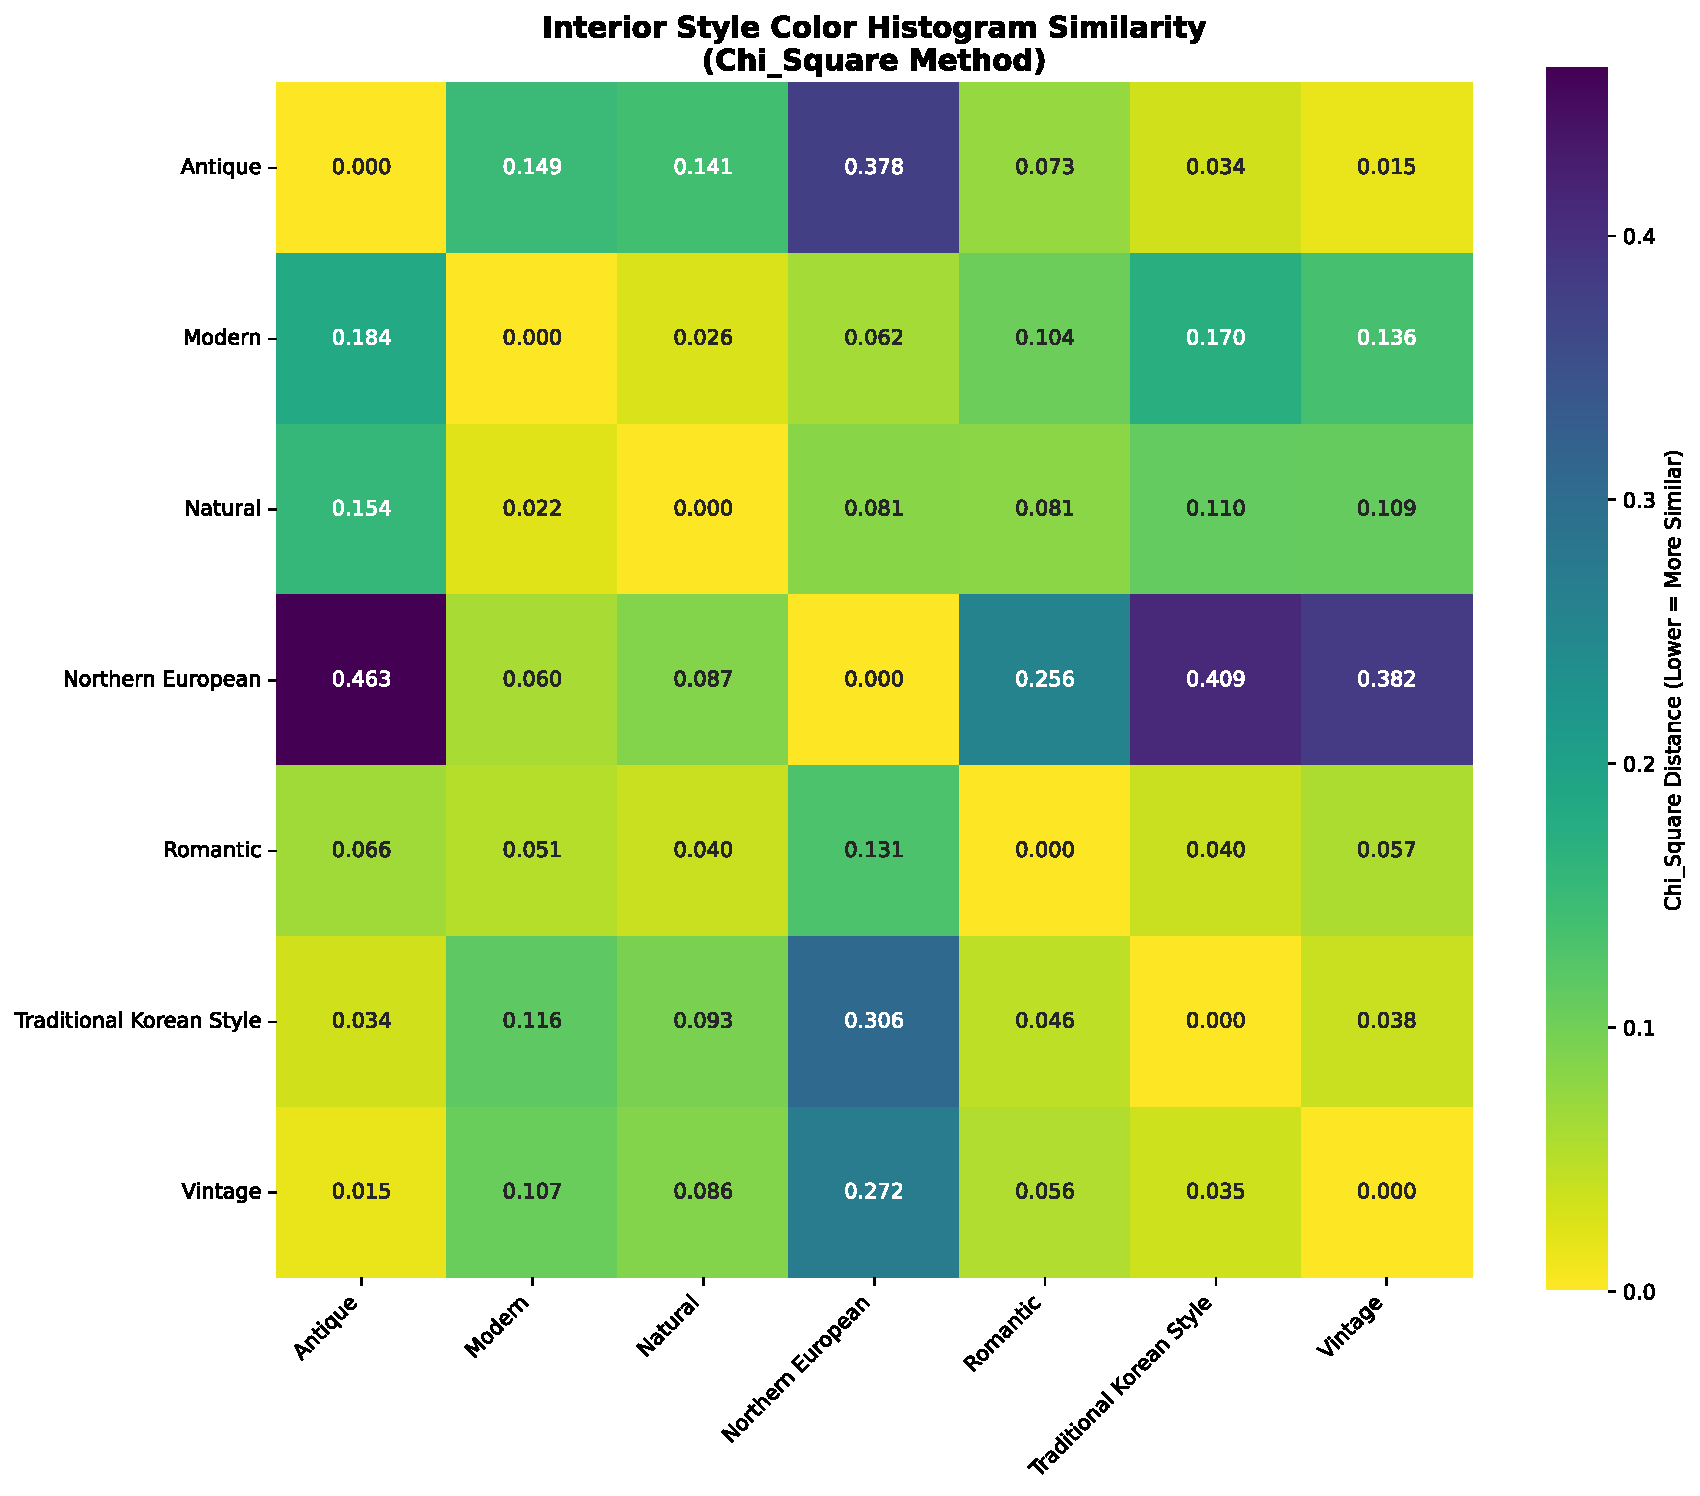
\includegraphics[width=\textwidth]{figures/rgb_chi_square_distance.pdf}
        \caption{Chi-Square Distance in RGB Space}
        \label{fig:rgb_chi_square_distance}
    \end{subfigure}
    \begin{subfigure}[b]{0.45\textwidth}
        \centering
        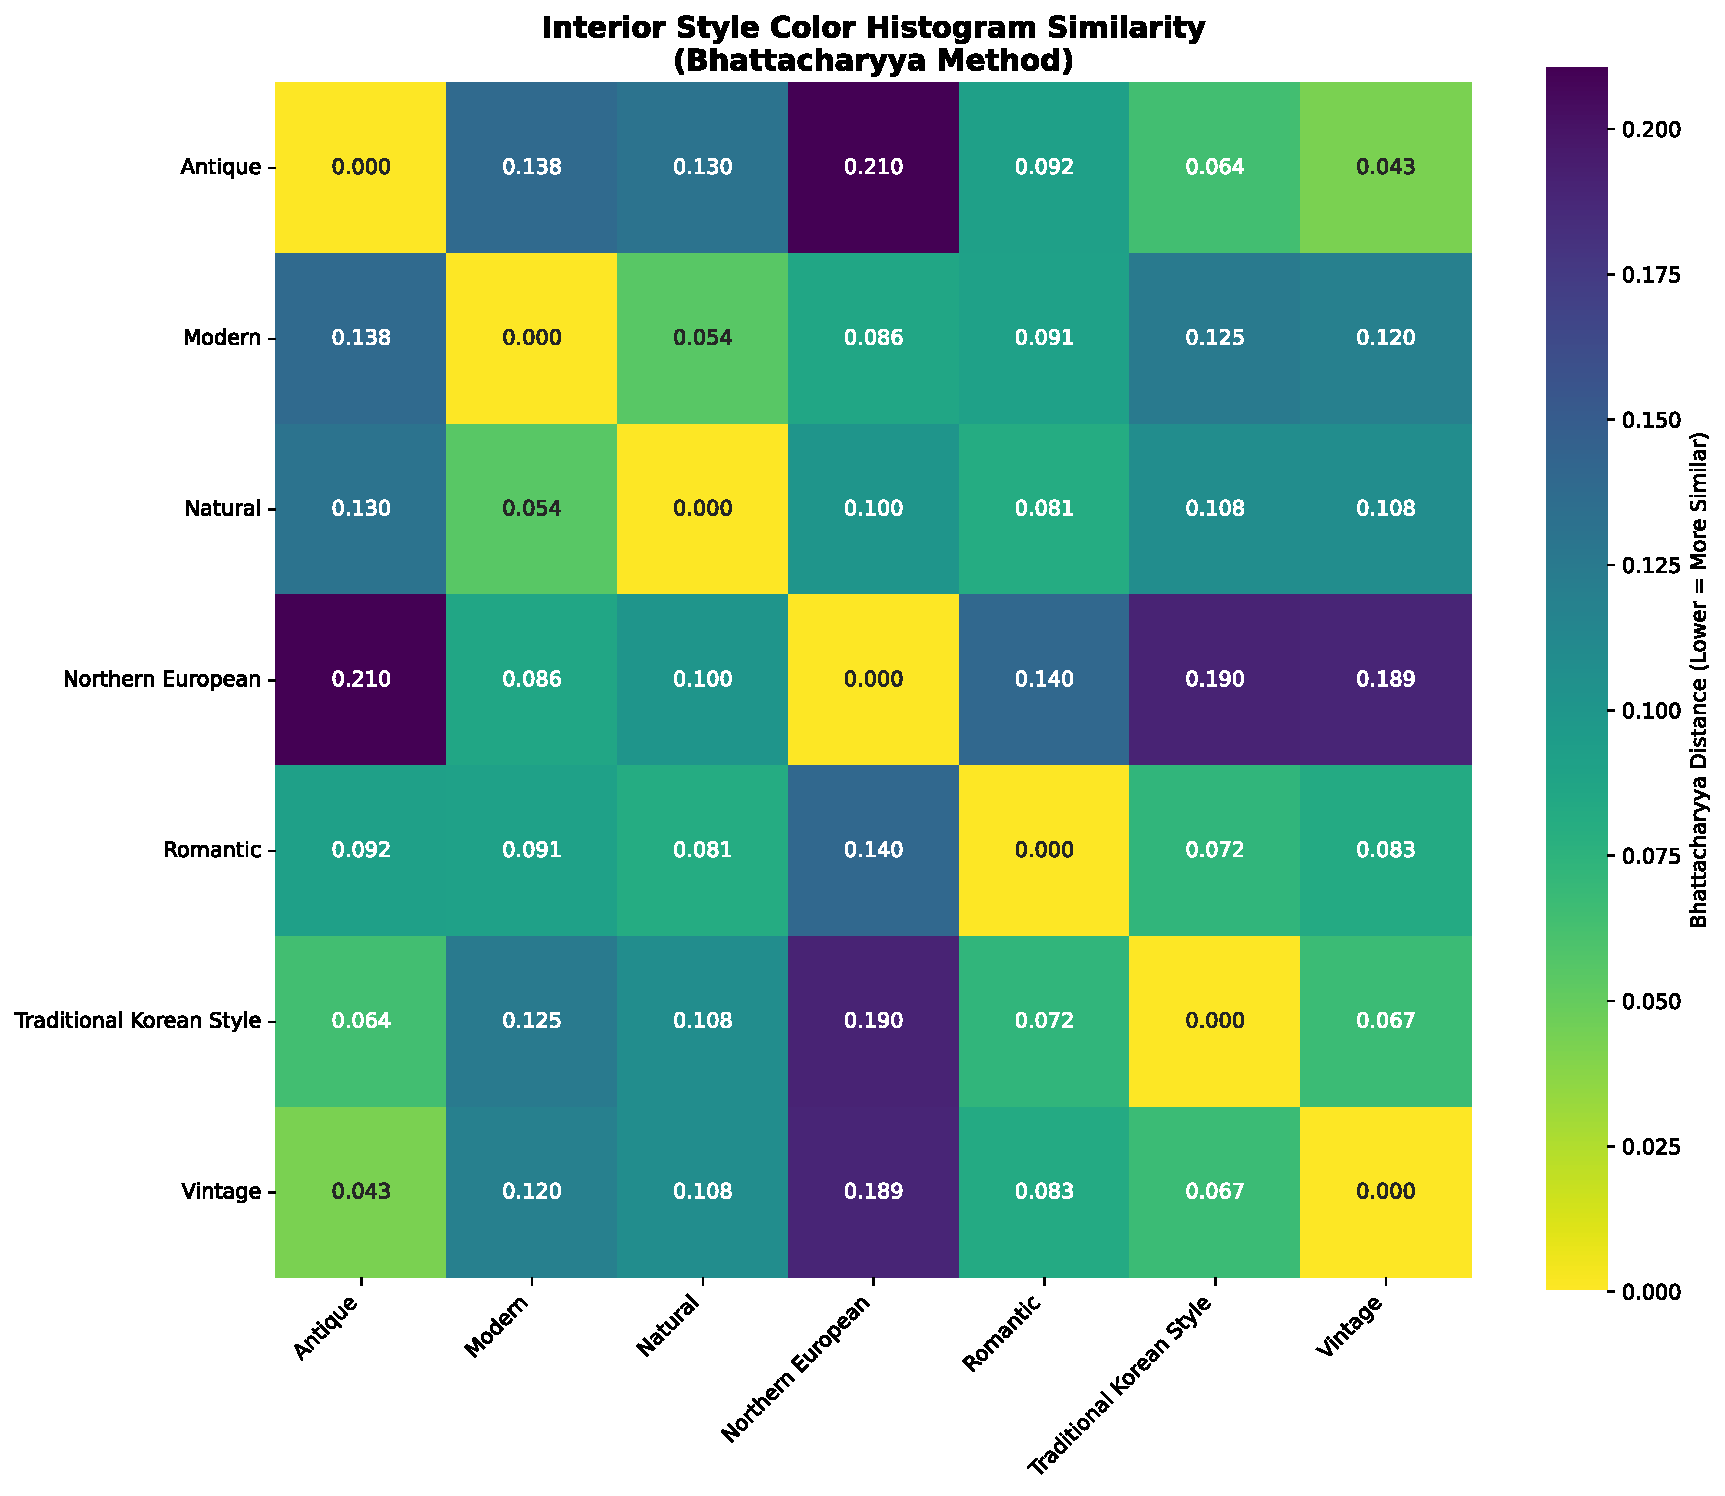
\includegraphics[width=\textwidth]{figures/rgb_bhattacharyya_distance.pdf}
        \caption{Bhattacharyya Distance in RGB Space}
        \label{fig:rgb_bhattacharyya_distance}
    \end{subfigure}
    \caption{Distance Comparison in RGB Space}
    \label{fig:rgb_distance_comparison}
\end{figure}
Antique와 Vintage는 두 거리 계산 방법 모두에서 가장 유사한 것으로 나타났고, Antique와 Northern European은 두 거리 계산 방법 모두에서 가장 유사하지 않은 것으로 나타났다.
전반적으로 Romantic이 다른 모든 스타일들과 대부분 유사한 것으로 나타났고, Nortern European이 다른 스타일들과 가장 유사하지 않은 것으로 나타났다.
이외에도 Traditional Korean Style은 Vintage와 가장 유사한 것으로 나타났고, Modern과 Natural은 서로 가장 유사한 것으로 나타났다.
비대칭 카이제곱 거리를 사용했기 때문에 각 스타일 간의 거리가 대칭적이지 않다는 점에 유의해야 한다.

\subsubsection{Color Histogram in HSV Space}
\begin{figure}[htbp]
    \centering
    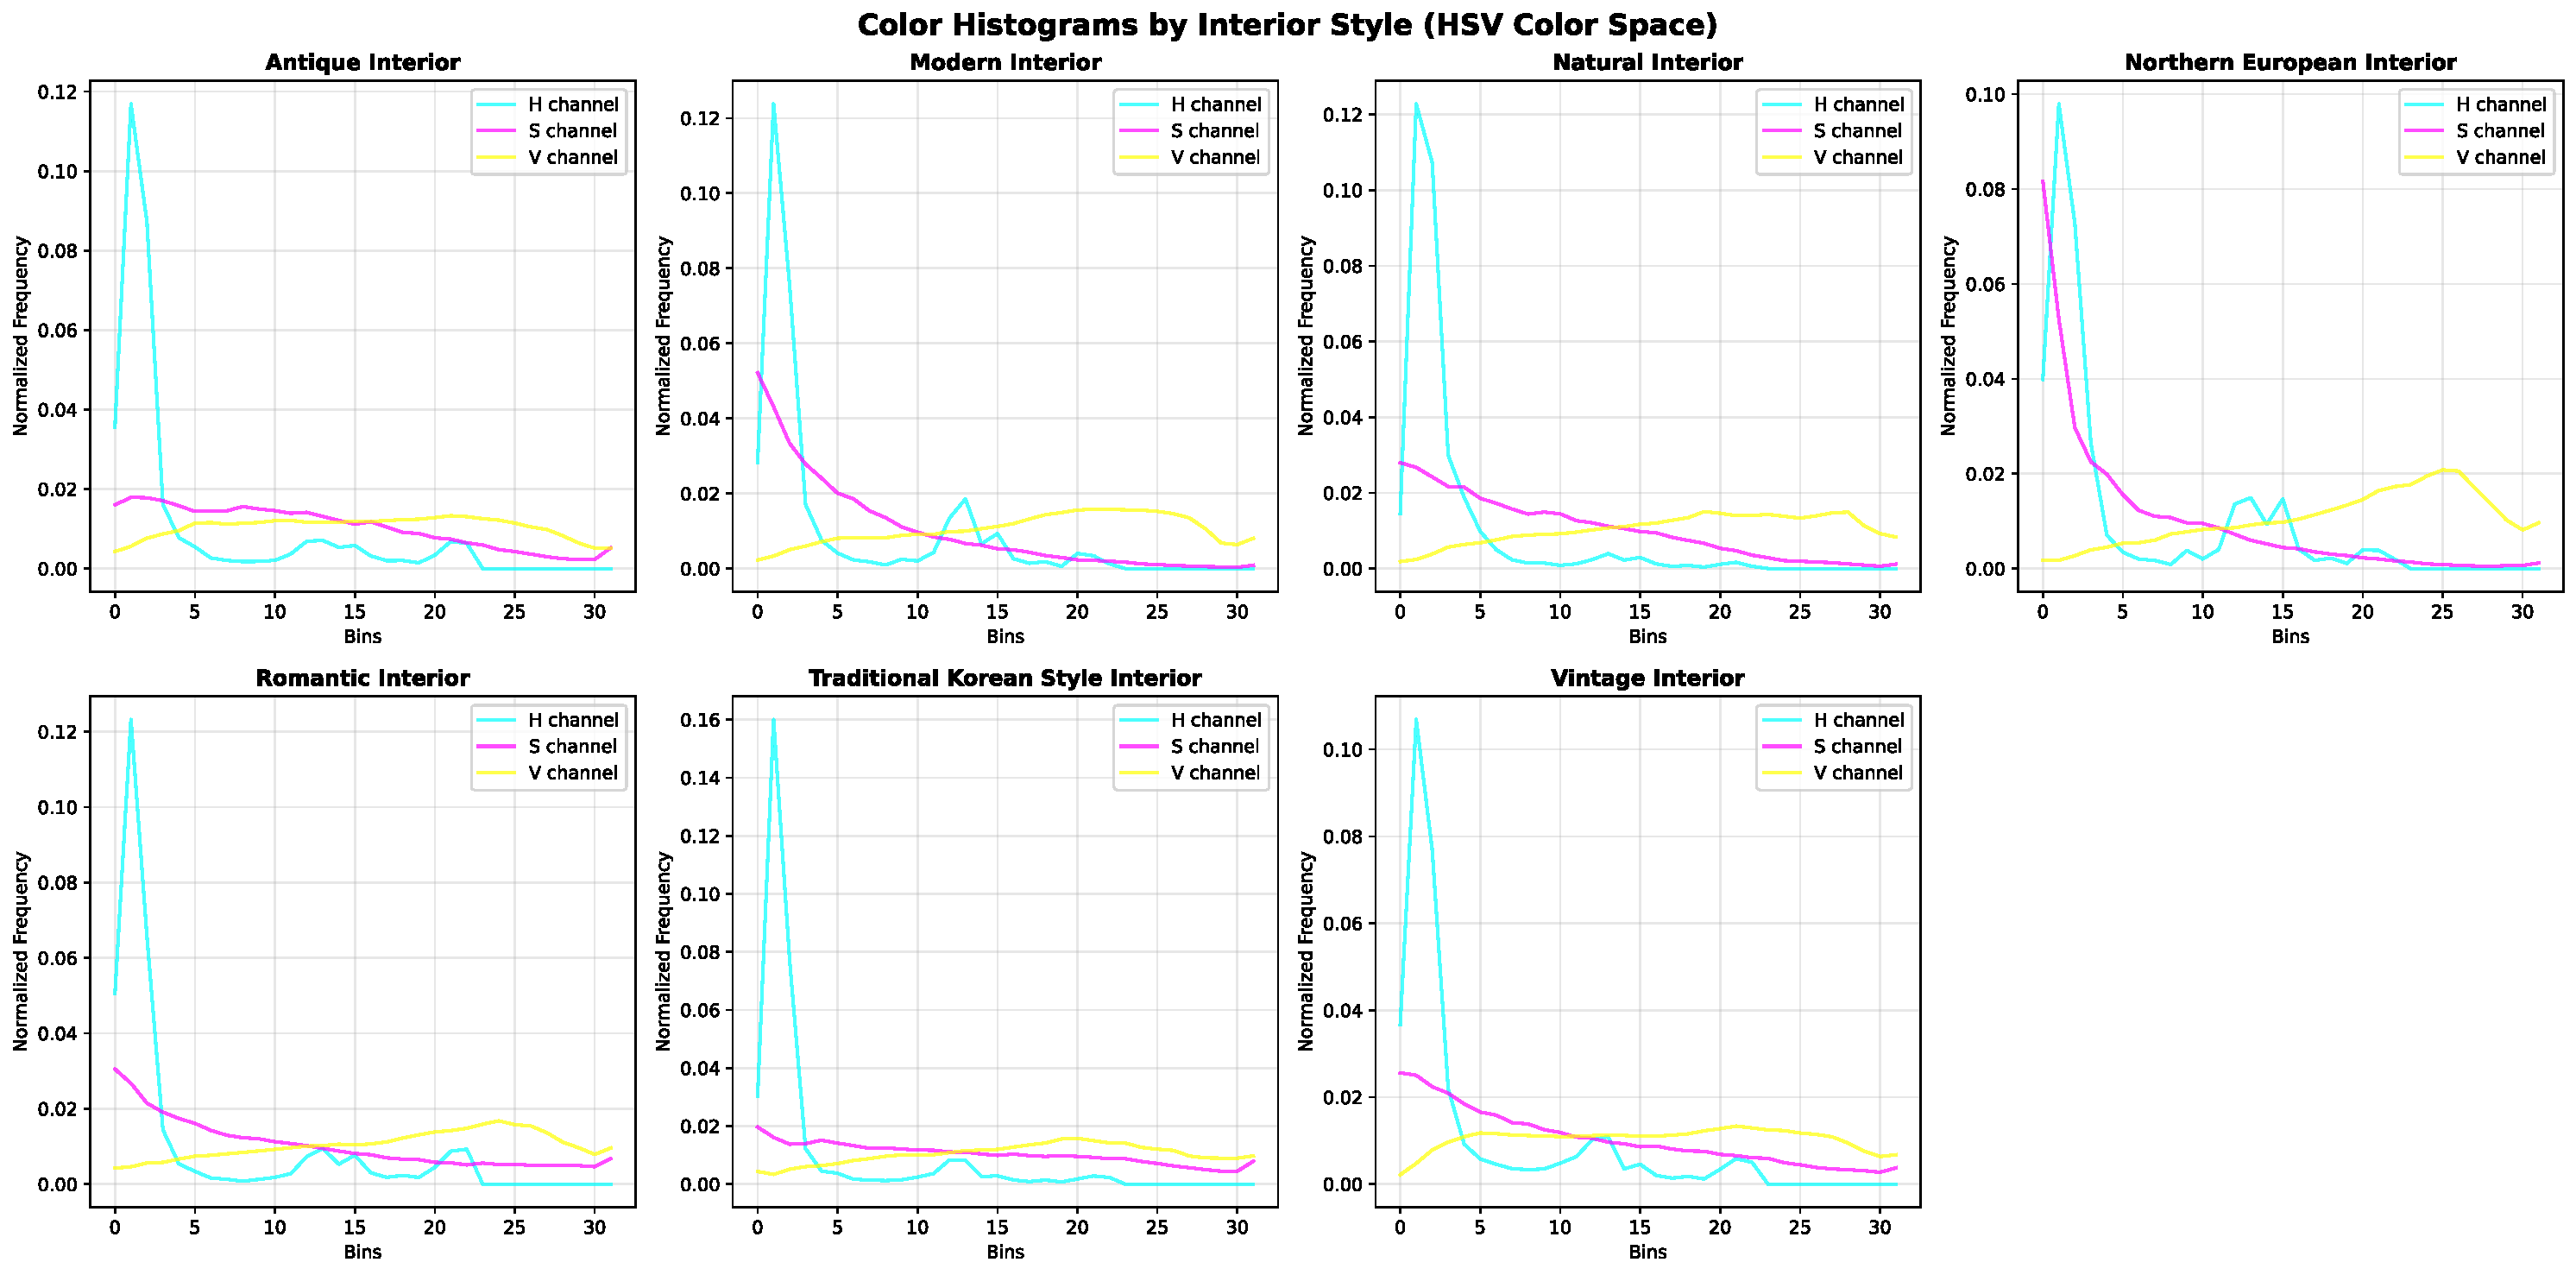
\includegraphics[width=0.8\textwidth]{figures/hsv_color_histogram.pdf}
    \caption{Color Histogram in HSV Space}
    \label{fig:hsv_color_histogram}
\end{figure}
HSV 색 공간에서의 색 히스토그램을 추출한 결과는 위와 같다. RGB 색 공간과 동일하게 카이제곱 거리와 바타차리야 거리를 계산하여 비교하였다.
\begin{figure}[htbp]
    \centering
    \begin{subfigure}[b]{0.45\textwidth}
        \centering
        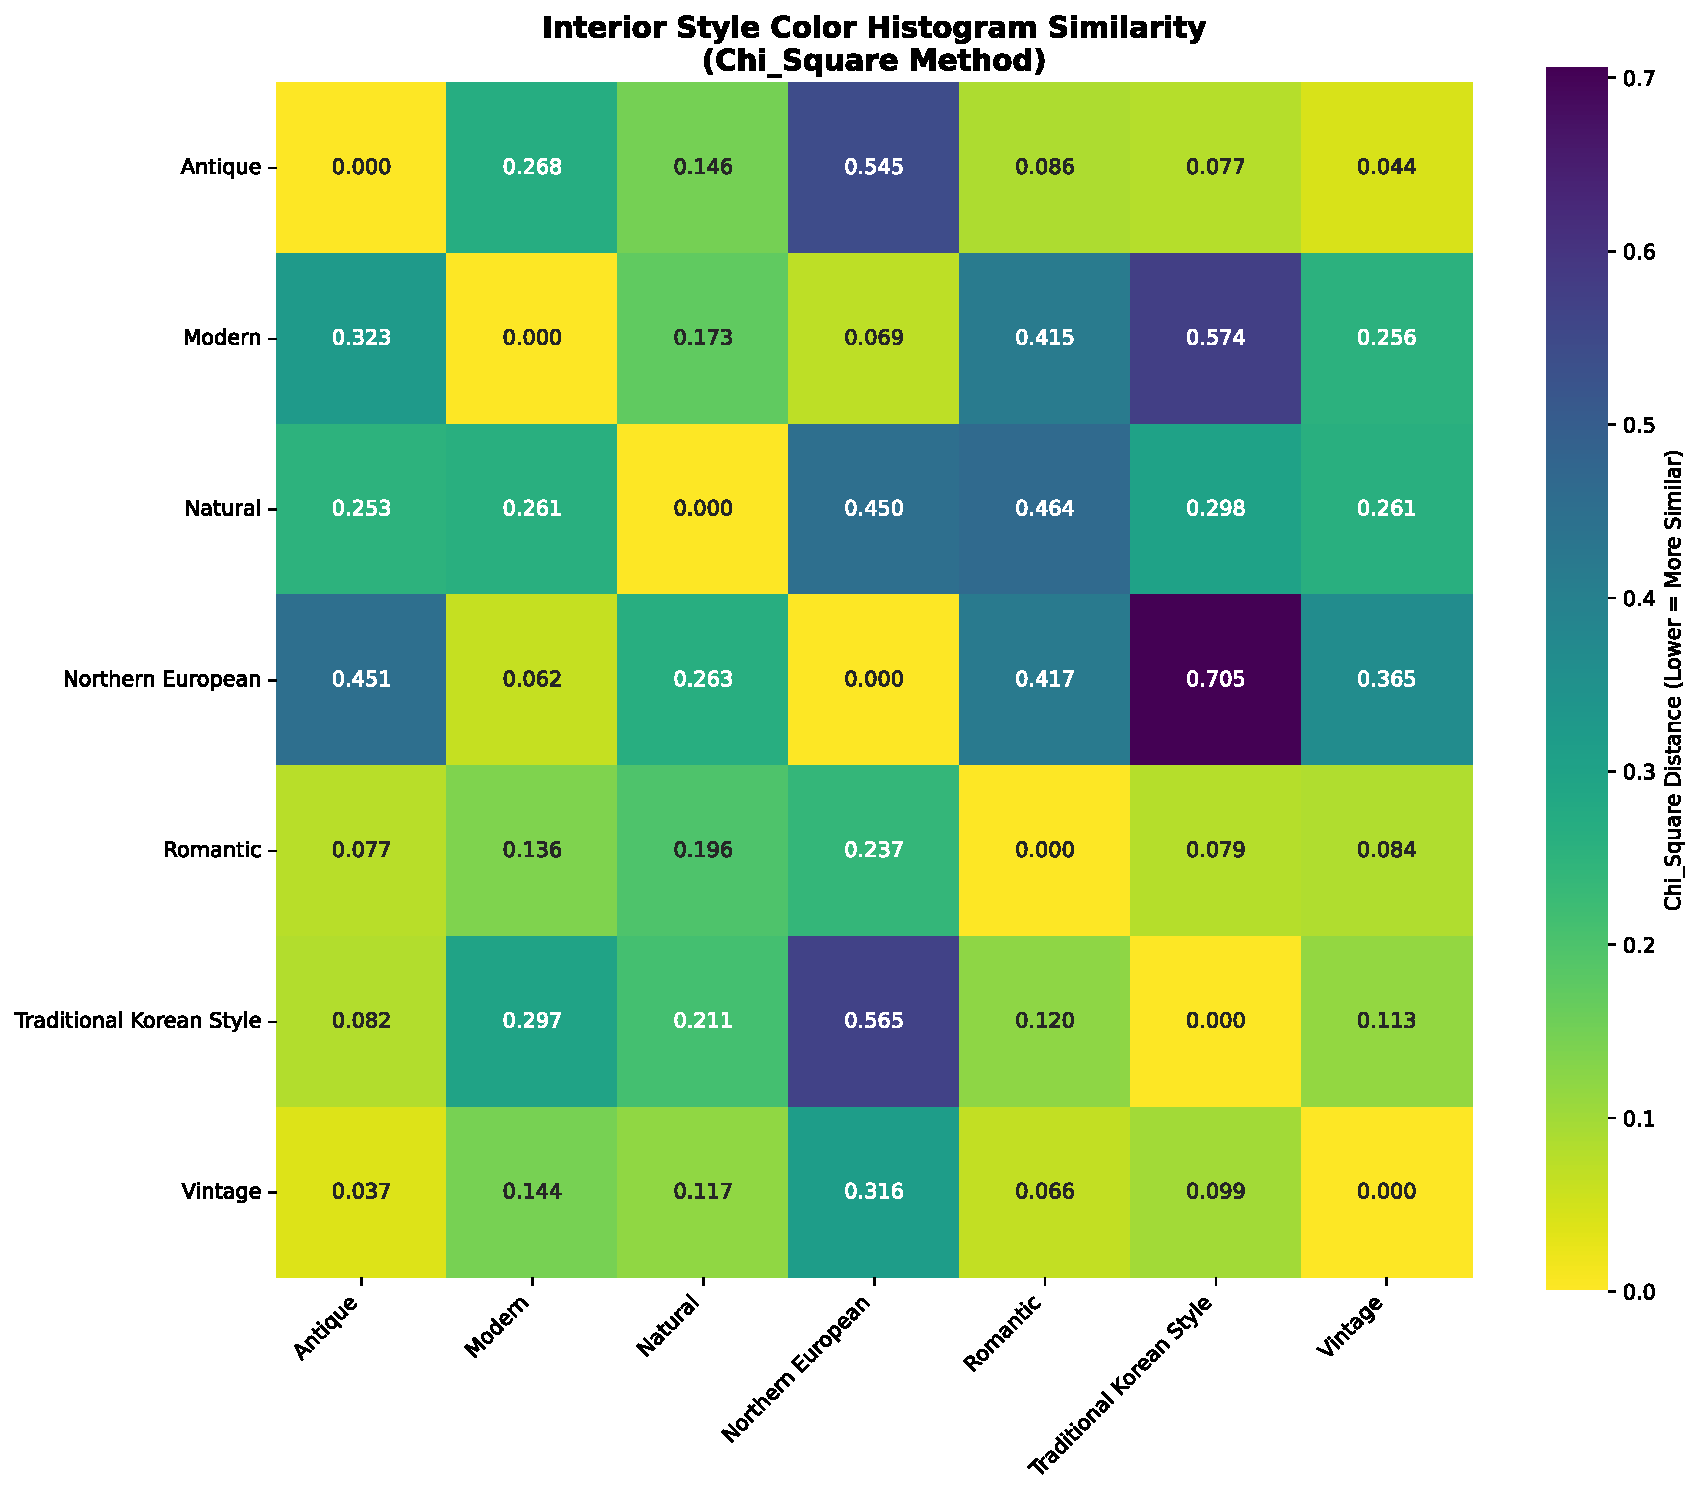
\includegraphics[width=\textwidth]{figures/hsv_chi_square_distance.pdf}
        \caption{Chi-Square Distance in HSV Space}
        \label{fig:hsv_chi_square_distance}
    \end{subfigure}
    \begin{subfigure}[b]{0.45\textwidth}
        \centering
        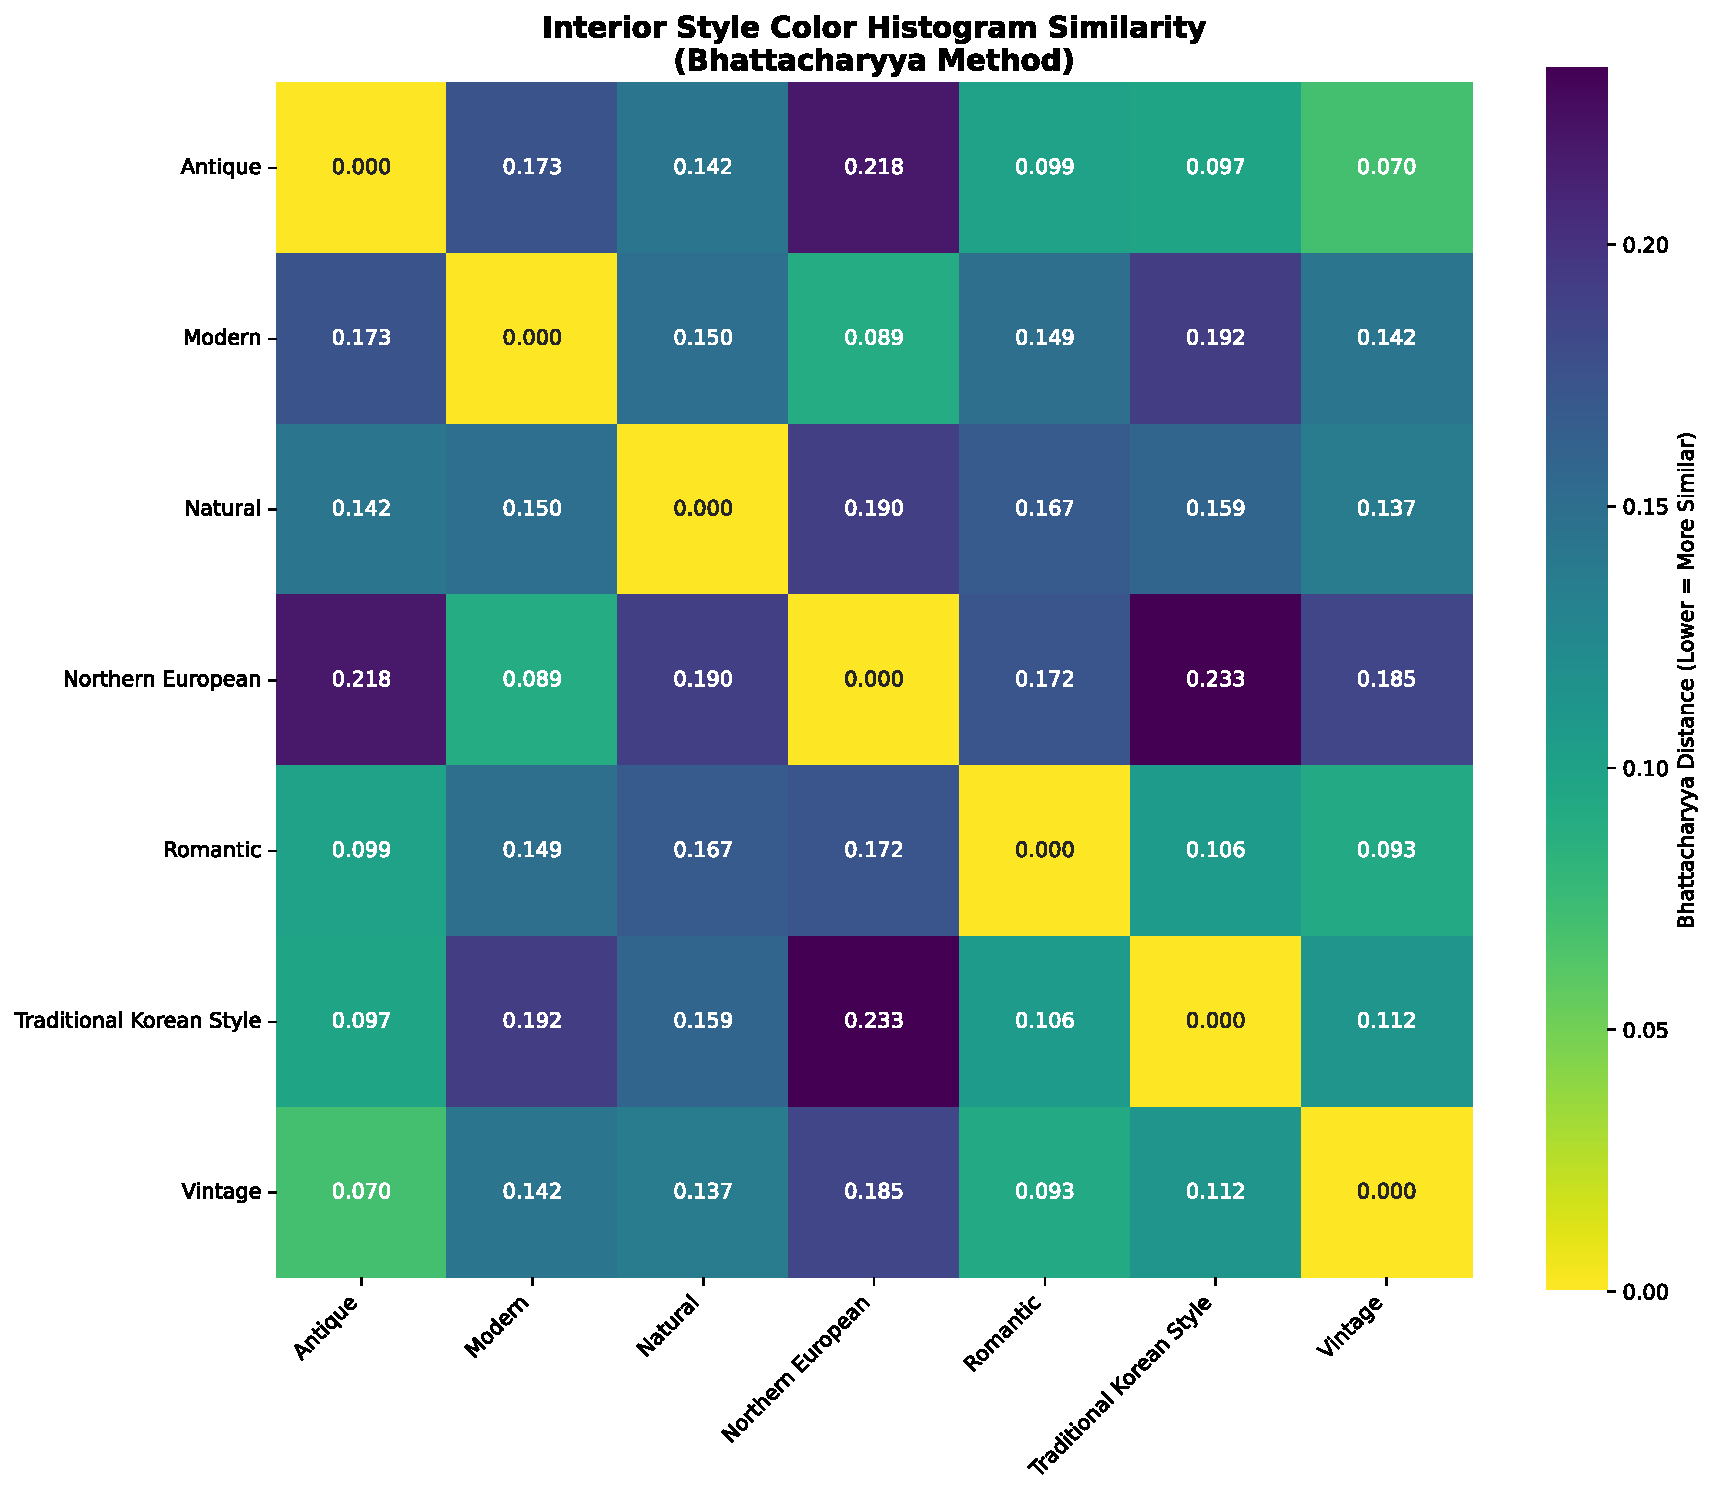
\includegraphics[width=\textwidth]{figures/hsv_bhattacharyya_distance.pdf}
        \caption{Bhattacharyya Distance in HSV Space}
        \label{fig:hsv_bhattacharyya_distance}
    \end{subfigure}
    \caption{Distance Comparison in HSV Space}
    \label{fig:hsv_distance_comparison}
\end{figure}

RGB 색 공간과는 다르게 Nortern European과 Traditional Korean Style이 가장 유사하지 않은 것으로 나타났고, Antique와 Vintage는 두 거리 계산 방법 모두에서 가장 유사한 것으로 나타났다.
전반적으로 Romantic이 다른 모든 스타일들과 대부분 유사한 것으로 나타났고, RGB 색 공간과는 다르게 Modern, Natural, Nortern European이 다른 색들과 거리가 먼 것으로 나타났다.

\subsection{3D Object Generation}
사용자가 입력한 텍스트를 기반으로 3D 가구 객체를 제대로 생성하는지 확인하기 위해서 정성적인 확인 방법을 사용하였다. 

\subsection{Size Prediction}

\section{Results}

\section{Conclusion}

\bibliographystyle{unsrt}
\bibliography{references}

\end{document}